
\begin{frame}{第五章}
    \begin{itemize}
        \item 二项式系数及相关恒等式
        \item 练习，练习，练习！
        \item 差分和二项式反演
        \item 生成函数初步
    \end{itemize}
\end{frame}
\begin{frame}{第五章习题}
    接下来两周内，阅读 5.1-5.4。第一周至少需要读完 5.1-5.2 并把 5.2 中所有练习自己推一遍。
    
    习题中需要写下来的（需要对每道题自行判断目前学完的东西能不能让你完成这道题）：
    
    2 3 4 5 8 14 15 16 35 36 37 40 41 43 45 46 47 59 61 63 64 67 70 71 73 74 76 77 79
    
\end{frame}
\begin{frame}{组合计数}
    \begin{itemize}
        \item 加法原理：$|A\uplus B|=|A|+|B|$
        \item 乘法原理：$|A\times B|=|A||B|$
        \begin{itemize}
            \item 扩展的乘法原理：假设 $S$ 是 $A\times V$ 的一个子集。如果对每个 $x\in A$，都有 $\#\{y:(x,y)\in S\}=m$，则 $|S|=m|A|$
        \end{itemize}
        \item 减法（容斥）原理：$|A-B|=|A|-|A\cap B|$
        \item 除法原理：假设 $S$ 是 $A\times V$ 的一个子集。如果对每个 $x\in A$，$\#\{y:(x,y)\in S\}$ 都相等，则 $\#\{y:(x,y)\in S\}=|S|/|A|$
    \end{itemize}
\end{frame}
\begin{frame}{球与盒子}
    洛谷 P5824 十二重计数法（由于本题实际需要 FFT，我们只列式子）
\end{frame}
\begin{frame}{I 和 II}
    逐球考虑，容易用乘法原理计数。得到 $f_{\mathrm{I}}(n,m)=m^n$ 和 $f_{\mathrm{II}}=m^{\underline n}$。

    如果逐盒子考虑呢？对于 I，枚举每个盒子里的球数得到
    $$
    \begin{aligned}
    &\sum_{i_1+i_2+\cdots+i_m=n}\binom{n}{i_1}\binom{n-i_1}{i_2}\binom{n-i_1-i_2}{i_3}\cdots\binom{n-i_1-\cdots-i_{m-1}}{i_m}\\
    &=\sum_{i_1+i_2+\cdots+i_m=n}\frac{n!}{i_1!i_2!\cdots i_m!}\\
    &=(1+1+\cdots+1)^n=m^n.
    \end{aligned}
    $$

    对于 II，类似计算得到 
    $$
    \sum_{i_1+i_2+\cdots+i_m=n;i_1,i_2,\ldots,i_m\le 1}n!=\binom{m}{n}n!=m^{\underline{n}}.
    $$
\end{frame}
\begin{frame}{III}
    逐球考虑难以处理限制，不过我们可以先把限制容斥掉。容斥后，如果强制了 $i$ 个空盒子，那么就变成 $f_{\mathrm{I}}(n,m-i)$。所以
    $$
    f_{\mathrm{III}}(n,m)=\sum_i\binom{m}{i}(-1)^i f_{\mathrm{I}}(n,m-i)=\sum_{i}\binom{m}{i}(-1)^i (m-i)^n.
    $$

    也可以逐盒考虑，这样就是
    $$
    \sum_{i_1+i_2+\cdots+i_m=n;i_1,\ldots,i_m\ge 1}\frac{n!}{i_1!i_2!\cdots i_m!}.
    $$
    仍然需要容斥掉 $i_j\ge 1$ 来计算。
\end{frame}
\begin{frame}{生成函数}
    考虑关于 $n$ 的 EGF。在这三种情况下，一个盒子的 EGF 分别为 $e^x$、$1+x$ 和 $e^x-1$，所以整个 EGF 分别是 $e^{mx}$、$(1+x)^m$ 和 $(e^x-1)^m$。
\end{frame}
\begin{frame}{标号（一）}
    有区别/可区分/有标号/互不相同都指向相同的概念。一般来说，有标号是最通用和方便的说法。

    球与盒子均互不相同的情况具有完整的标号，可以逐球考虑/逐盒子考虑来计数。

    在球互不相同、盒子相同时，盒子的任意排列被视为同一种方案（等价类）。此时，常见的处理方法是\textbf{强制}一个顺序。
        \begin{itemize}
            \item 注意到当盒子均非空时，每个等价类的大小都为 $m!$（也就是盒子的任意排列都对应一种不同的方案）。所以 $f_{\mathrm{VI}}(n,m)=\frac{1}{m!}f_{\mathrm{III}}(n,m)$。
            \item 有空盒子的情况则更复杂一些，因为空盒子的不同排列即使在盒子有标号时对应的也是同一种方案。假设有 $m-k$ 个空盒子，那么等价类大小是 $\frac{1}{\binom{m}{m-k} k!}=\frac{1}{m^{\underline{k}}}$。
        \end{itemize}
\end{frame}
\begin{frame}{IV, V 和 VI}
    由于盒子无区别，我们可以强制一个顺序。例如，按照每个盒子里装的球的最小标号升序排序（空盒子视为 $0$）。那么对于 IV，我们可以想象前面有一些空盒子，然后后面是一个 VI。所以
    $$
    f_{\mathrm{IV}}(n,m)=\sum_{i=0}^m f_{\mathrm{VI}}(n,i).
    $$

    对于 V，唯一的一种排法就是 $m-n$ 个空盒子后面按顺序排着装 $1,2,\ldots,n$ 的盒子。所以 $f_{\mathrm{V}}(n,m)=[n\le m]$。或者通过上一页中对等价类的分析，我们也可以发现 $f_{\mathrm{V}}(n,m)=\frac{1}{m^{\underline{n}}}f_{\mathrm{II}}(n,m)$。

    对于 VI，我们在上一页中已经得到 $f_{\mathrm{VI}}=\frac{1}{m!}f_{\mathrm{III}}$。事实上，这就是第二类斯特林数 $n\brace m$ 的一种定义。代入 III 的结果就得到
    $$
    {n\brace m}=\frac{1}{m!}\sum_i\binom{m}{i}(-1)^i(m-i)^n.
    $$
\end{frame}
\begin{frame}{标号（二）}
    在球相同、盒子互不相同时，有标号球退化为无标号的“单位”，也就是只关心每个盒子里装球的\textbf{个数}。
    \begin{itemize}
        \item 此时的一个等价类大小为 $\frac{n!}{n_1!\cdots n_m!}$，其中 $n_i$ 为第 $i$ 个盒子里的球数。
        \item 因为不同等价类大小不同，除法原理无法在此应用。
    \end{itemize} 

    在球相同、盒子也相同时，盒子的任意排列被视为同一种方案。此时可以强制按照盒子中装的球数来排序。
    \begin{itemize}
        \item 此时的一个等价类在前一个问题中具有大小 $\frac{m!}{m_0!m_1!m_2!\cdots m_n!}$，其中 $m_i$ 表示装了 $i$ 个球的盒子个数。
        \item 同样因为不同等价类大小不同，除法原理无法在此应用。
    \end{itemize}
\end{frame}
\begin{frame}{VII, VIII 和 IX}
    我们可以通过如下操作建立 VII 与 IX 的双射：对于每个合法的 VII 方案，在每个盒子里放一个球即可得到一个合法的 IX 方案，并且这是一个单射；反之，对于每个合法的 IX 方案，在每个盒子里拿走一个球即可得到一个合法的 VII 方案，而这同样是一个单射。所以我们得到 $f_{\mathrm{VII}}(n,m)=f_{\mathrm{IX}}(n+m,m)$。

    对于 IX，我们可以使用称为“隔板法”的双射：在 $n$ 个球之间插 $m-1$ 个隔板，这与 IX 的方案有一一对应。而前者的方案数显然是 $\binom{n-1}{m-1}$，所以 $f_{\mathrm{IX}}(n,m)=\binom{n-1}{m-1}$。这样我们也得到 $f_{\mathrm{VII}}(n,m)=\binom{n+m-1}{m-1}$。（也可以枚举第一个盒子放了几个球，然后使用我们以前学过的方法处理递推式）

    对于 VIII，我们可以考虑哪些盒子装了球，这有 $\binom{m}{n}$ 种方案。或者，我们也可以使用上一页中的等价类大小分析来得到 $f_{\mathrm{VIII}}(n,m)=f_{\mathrm{II}}(n,m)/n!$。
\end{frame}
\begin{frame}{生成函数}
    在这三种情况下，一个盒子的 OGF 分别为 $\frac{1}{1-x}$、$1+x$ 和 $\frac{x}{1-x}$。所以总的 OGF 分别为 $\frac{1}{(1-x)^m}$、$(1+x)^m$ 和 $\frac{x^m}{(1-x)^m}$。

    不难发现生成函数处理盒子有区别的情况是方便的。
\end{frame}
\begin{frame}{X, XI 和 XII}
    对于 XI，我们可以使用和 V 同样的分析，或者也可以使用前面的等价类大小分析来得到同样的 $f_{\mathrm{XI}}=[n\le m]$。

    对于 X 和 XII，我们可以类比 VII 与 IX 来得到 $f_{\mathrm{X}}(n,m)=f_{\mathrm{XII}}(n+m,m)$。

    \vspace{0.5em}

    \begin{columns}[T, onlytextwidth]

    \begin{column}{0.8\textwidth}
    对于 X，这是一个拆分数类型的问题。此类问题的直观理解如下：把每个球画成一个点，把一个盒子里装的球画成一行的点，不同盒子画在不同行并对齐，强制盒子里装的球数从上往下不降。这样得到的点阵被称为 \textbf{Ferrers} 图。例如，右图就是 2, 3, 5, 5 的 Ferrers 图。

    \vspace{1em}

    从这个图中我们可以注意到其行和列是\textbf{对称}的，而列的组合意义是盒子的容量限制。所以，使用不超过 $m$ 个盒子、容量无限制的方案数等于盒子数量无限制、每个盒子容量不超过 $m$ 的方案数。
    \end{column}

    \begin{column}{0.2\textwidth}
        \vspace{1cm}
    
        \centering

    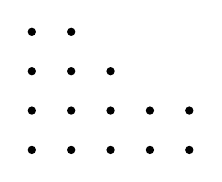
\begin{tikzpicture}[scale=0.5]
        % Partition: change this list
        \def\partition{2,3,5,5}
    
        \foreach \y [count=\i] in \partition {
            \foreach \x in {1,...,\y} {
                \fill (\x, {5-\i}) circle (3pt);
            }
        }

    \end{tikzpicture}

    \end{column}
    \end{columns}
\end{frame}
\begin{frame}{Ferrers 图：DP I}
            下面省略 $f_{\mathrm{X}}$ 的下标 X，即写作 $f(n,m)$。首先，我们可以通过枚举最左边有几列高度为 $m$，得到
            $$
            f(n,m)=\sum_{i\ge 0}f(n-im,m-1).
            $$ 
            通过相减抵消求和，可以得到 $f(n,m)=f(n-m,m)+f(n,m-1)$，这是一个 $O(nm)$ 的 dp。或者，我们也可以枚举最左边一列的高度，再通过相减抵消求和得到相同的 dp。
            $$
            f(n,m)=\sum_{i\le m}f(n-i,i)=f(n,m-1)+f(n-m,m)
            $$

            这个 dp 还有另一个理解：考虑行数够不够 $m$，如果不够那么是 $f(n,m-1)$，如果够那么可以把第一列删掉，这样是 $f(n-m,m)$。总之，如果 $m\le \sqrt{n}$，我们就得到了一个 $O(n\sqrt{n})$ 的做法。
\end{frame}
\begin{frame}{Ferrers 图：DP II}
            如果 $m>\sqrt{n}$，我们可以想象 Ferrers 图的结构：左边有若干高度 $>\sqrt{n}$ 的列（不超过 $\sqrt{n}$ 个），右边是高度不超过 $\sqrt{n}$ 的列。记 $B=\lfloor \sqrt{n}\rfloor+1$ 为左边的列高度的可能最小值，后面的讨论中都假设 $B$ 是独立于 $n$ 的变量。
            
            如果我们可以在 $O(n^2/B)$ 的时间内计算出所有 $g_B(i)$，表示每列高度都在 $[B,m]$ 内的 $i$ 个点的 Ferrers 图的数量，那么就可以枚举左右的点数计算答案：
            $$
            f(n,m)=\sum_{i}g_B(n-i)f(i,B-1).
            $$      

            而 $f(i,B-1)$ 可以通过上一页的 dp 在 $O(nB)=O(n\sqrt{n})$ 时间内计算。
\end{frame}            
\begin{frame}
            现在来考虑 $g_B$ 的计算。设 $g(n,k)$ 表示列数恰好为 $k$ 且每列高度都在 $[B,m]$ 内的 Ferrers 图数量，则 $k\le n/B$。我们考虑有没有高度为 $B$ 的列。如果有，那么这样的方案数为 $g(n-B,k-1)$；如果没有（也就是都 $>B$），那么我们可以把最后一行删去，所以方案数是列数恰好为 $k$ 且每列高度都在 $[B,m-1]$ 内的 $n-k$ 个点的 Ferrers 图数量。而这个可以用高度都在 $[B,m]$ 内的方案数减去最高高度恰好为 $m$ 的方案数来计算，其中前者就是 $g(n-k,k)$，而后者可以通过删掉第一列得到 $g(n-k-m,k-1)$。所以
            $$
            g(n,k)=g(n-B,k-1)+g(n-k,k)-g(n-k-m,k-1).
            $$ 
            再对 $k$ 做一下前缀和就可以计算出 $g_B(n)$。
\end{frame}
\begin{frame}{对全部的 $n$ 计算}
    如果直接卷积，那么需要 $O(n^2)$ 时间。然而，如果把 $f(i,B-1)$ 作为初值来做 $g$ 的 dp，那么就可以在 $O(n\sqrt{n})$ 时间内算出全部的 $f(n,m)$。或者说，现在 $g(n,k)$ 的含义变为：\textbf{额外列数}恰好为 $k$ 的 Ferrers 图数量，其中额外列指的是这些高度在 $[B,m]$ 内的列。转移和之前是相同的，只是初值变成了 $f(i,B-1)$。
\end{frame}
\begin{frame}{Ferrers 图：正方形}
    另一种计算 $f(n,m)$ 的方法是考虑包含左下角的极大正方形。假设这个正方形的边长是 $i$，那么这个正方形上面的部分就是一个高度不超过 $m-i$、宽度不超过 $i$ 的 Ferrers 图，右边的部分是一个高度不超过 $i$ 的 Ferrers 图，而正方形本身提供了 $i^2$ 个点，所以 $i\le \sqrt{n}$。上面和右边的部分都可以类似前面的 dp 计算。

    可能也可以用上一页的手法算出所有 $n$ 的结果。
\end{frame}
\begin{frame}{Ferrers 图：生成函数}
    考虑高为 $i$ 的行有几个，不难写出生成函数
    $$
    \prod_{i=1}^m\frac{1}{1-x^i}.
    $$
    可以通过 $\ln-\exp$ 做到 $O(n\log n)$，或者使用 q-analog 理论得到若干种不需要 FFT 的 $O(n\sqrt{n})$ 做法。
\end{frame}
\begin{frame}{变量计数}
    对于整数 $x_1,\ldots,x_m\ge 0$，求

    \begin{itemize}
        \item $x_1+x_2+\cdots+x_m=n$ 的方案数
        \item 在上一条的基础上，加上 $l_i\le x_i< r_i$ 的限制
        \item $x_1\le x_2\le\cdots\le x_{m-1}\le x_m=n$ 的方案数
        \item 在上一条的基础上，加上 $l_i\le x_i-x_{i-1}< r_i$ 的限制（设 $x_0=0$）
    \end{itemize}
\end{frame}
\begin{frame}
    第一个问题和之前的 VII 是相同的。

    通过换元 $y_i=x_i-x_{i-1}$，可以发现第三（四）个问题和第一（二）个问题是相同的。（事实上，我们以前已经通过和式处理的手法计算过第三个问题）

    对于第二个问题，先考虑只有下界 $x_i\ge l_i$ 的情况。通过换元 $y_i=x_i-l_i$，我们可以将其变成第一个问题（$n$ 变成 $n-\sum_i l_i$）。

    现在，我们可以不失一般性地假设 $l_i=0$。然后我们可以通过容斥把上界 $r_i$ 变成下界。
\end{frame}
\begin{frame}
    $$
    \begin{aligned}
    &\sum_{x_1+x_2+\cdots+x_m=n}\prod_i [x_i<r_i]\\
    &=\sum_{x_1+x_2+\cdots+x_m=n}\prod_i(1-[x_i\ge r_i])\\
    &=\sum_{x_1+x_2+\cdots+x_m=n}\sum_{S\subseteq [m]}\prod_{i\in S}-[x_i\ge r_i]\\
    &=\sum_{S\subseteq [m]}\sum_{x_1+x_2+\cdots+x_m=n}\prod_{i\in S}[x_i\ge r_i]\\
    &=\sum_{S\subseteq [m]}(-1)^{|S|}\binom{n-\sum_{i\in S}r_i+m-1}{m-1}
    \end{aligned}
    $$
    接下来可以 $2^m$ 枚举 $S$ 来计算。
\end{frame}

\begin{frame}{背包}
    也可以枚举 $R=\sum_{i\in S}r_i$ 得到
    $$
    \begin{aligned}
    &\sum_{S\subseteq [m]}(-1)^{|S|}\binom{n-\sum_{i\in S}r_i+m-1}{m-1}\\
    &=\sum_R\binom{n-R+m-1}{m-1}\sum_{S\subseteq [m]}(-1)^{|S|}\left[\sum_{i\in S}r_i=R\right],
    \end{aligned}
    $$
    而后者可以背包计算：
    $$
    \begin{aligned}
    f_{m,R}&=\sum_{S\subseteq [m]}(-1)^{|S|}\left[\sum_{i\in S}r_i=R\right]\\
    &=\sum_{S\subseteq [m-1]}(-1)^{|S|+1}\left[r_m+\sum_{i\in S}r_i=R\right]+ \sum_{S\subseteq [m]}(-1)^{|S|}\left[\sum_{i\in S}r_i=R\right]\\
    &=-f_{m-1,R-r_m}+f_{m-1,R}.
    \end{aligned}
    $$
    这样是 $O(nm)$ 的。由于 $n\gg 2^m$ 也是常见的，所以要根据情况选择做法。

    另外，也可以通过生成函数和 $\ln-\exp$ 技巧做到 $O(n\log n)$。
\end{frame}
\begin{frame}{排列}
    $n$ 个数的环排列个数

    $k$ 种颜色的球，第 $i$ 种颜色的有 $n_i$ 个，求方案数

    P2476 [SCOI2008] 着色方案：同上，但是要求相邻颜色不相同

    *P6151 [集训队作业2019] 青春猪头少年不会梦到兔女郎学姐

    P5339 [TJOI2019] 唱、跳、rap和篮球
\end{frame}
\begin{frame}
    对于第一个问题，每个环排列通过转圈对应到 $n$ 个不同的排列，所以方案数是 $n!/n=(n-1)!$。

    对于第二个问题，每个等价类通过对同色球内部的排列对应到 $\prod_i n_i!$ 个不同的排列，所以方案数是 $\frac{n!}{\prod_i n_i!}$。或者，也可以一个颜色一个颜色放置，得到 
    $$
    \binom{n}{n_1}\binom{n-n_1}{n_2}\binom{n-n_1-n_2}{n_3}\cdots\binom{n-n_1-\cdots-n_{k-1}}{n_k}=\frac{n!}{\prod_i n_i!}.
    $$

    也就是多项式系数 $\binom{n}{n_1,\ldots,n_k}$
\end{frame}
\begin{frame}{数列}
    长为 $n$ 的字符集大小为 $m$ 的字符串，不能出现连续 $k$ 个相同字符，求方案数

    *P1393 Mivik 的标题：长为 $n$ 的字符集大小为 $m$ 的字符串，不能出现子串 $S$，求方案数

    P6076 [JSOI2015] 染色问题

    P4491 [HAOI2018] 染色
\end{frame}
\begin{frame}{第一个问题}
    做法一：设 $f_{i,j}$ 表示长为 $i$ 的字符串，目前结尾极长连续段长度为 $j$，且从来没有出现过连续 $k$ 个相同字符的方案数，则 $f_{i,j}=f_{i-1,j-1}(j>1)$ 以及 $f_{i,1}=\sum_{j<k} (m-1)f_{i-1,j}$。$O(nk)$ 直接做或者 $O(k^3\log n)$ 矩阵加速。

    做法二：设 $f_i$ 表示长为 $i$ 的字符串，且从来没有出现过连续 $k$ 个相同字符的方案数。那么首先考虑 $mf_{i-1}$，然后再减掉不合法的方案数。不合法的情况一定是最后 $k$ 个字符都相同，且倒数第 $k+1$ 个字符和后面的不同。最后 $k$ 个字符有 $m$ 种可能；对于前面的串，由对称性，以每种字符结尾的合法串的个数都是 $f_{i-k}/m$，所以不合法方案数总共是 $(m-1)f_{i-k}$，故 $f_i=mf_{i-1}-(m-1)f_{i-k}$。$O(n)$ 直接做或者 $O(k^2\log n)$ 甚至 $O(k\log k\log n)$ 线性递推。
\end{frame}
\begin{frame}
    做法三：容斥，考虑对于每个位置钦定以这个位置结尾有 $k$ 个连续相同字符。然而剩下的事情十分困难，我们只给出生成函数的解释。想象一下钦定之后的序列会长成什么样子：序列被分成若干段，每一段要么是一个未被钦定的字符，要么是因为若干个间距小于 $k$ 的钦定位置而连成的一个大同色连续段。将这个结构翻译成生成函数：前者是 $mx$，后者是 $\frac{-mx^k}{1+\sum_{i=1}^{k-1}x^i}$（注意每个钦定带来 $-1$ 的系数）。最后再套一层序列就得到
    $$
    \left(1-mx-\frac{-mx^k}{1+\sum_{i=1}^{k-1}x^i}\right)^{-1}=\frac{1-x^k}{1-mx+(m-1)x^k}.
    $$

    做法四：考虑先枚举所有极长连续段的长度 $l_1,\cdots,l_t$，其贡献为 $m(m-1)^{t-1}$。这样我们也可以直接写出生成函数 
    $$
    \frac{m}{m-1}\cdot \frac{1}{1-(m-1)\sum_{i=1}^{k-1}x^i}=\frac{m}{m-1}\cdot \frac{1-x}{1-mx+(m-1)x^k}
    $$

    两个生成函数看起来有微妙的不同，这是 $f_0$ 导致的。事实上，上面那个生成函数才是完全正确的，下面这个会导致 $f_0=m/(m-1)$。这两个分式对应的线性递推和做法二是相同的。
\end{frame}
\begin{frame}
    另外，也可以直接展开生成函数：
    $$
    \begin{aligned}
    &[x^n]\frac{1-x^k}{1-mx+(m-1)x^k}=[x^n]\frac{1}{1-mx}\cdot \frac{1-x^k}{1+\frac{(m-1)x^k}{1-mx}}\\
    &=[x^n]\frac{1-x^k}{1-mx}\sum_{i\ge 0}(-1)^i\left(\frac{(m-1)x^k}{1-mx}\right)^i\\
    &=\sum_{i\ge 0}(-1)^i(m-1)^i[x^n]\frac{(1-x^k)x^{ik}}{(1-mx)^{i+1}}\\
    &=\sum_{i\ge 0}(-1)^i(m-1)^i\left([x^{n-ik}]\frac{1}{(1-mx)^{i+1}}-[x^{n-(i+1)k}]\frac{1}{(1-mx)^{i+1}}\right)\\
    &=\sum_{i\ge 0}(-1)^i(m-1)^i\left(m^{n-ik}\binom{n-ik+i}{n-ik}-m^{n-(i+1)k}\binom{n-(i+1)k+i}{n-(i+1)k}\right)
    \end{aligned}
    $$
    $i>n/k$ 后的项都是 $0$。每一个组合数都可以 $O(i)=O(n/k)$ 计算，总复杂度 $O((n/k)^2)$。

    上面这种手法是常用的，即把分式写作 $\frac{1}{A(x)-B(x)}=\frac{1}{A(x)}\frac{1}{1-B(x)/A(x)}$ 然后展开。
\end{frame}
\begin{frame}{第二个问题}
    前面的容斥做法可以扩展到一般的禁止子串 $S$，只需要重新刻画由若干个间距小于 $k=|S|$ 的钦定位置而连成的一个大固定串。这样的东西形如 $S$ 后面跟着若干个 $S$ 的长度小于 $k$ 的周期。所以总的生成函数就是
    $$
    \left(1-mx-\frac{-x^k}{1+c(x)}\right)^{-1},
    $$
    其中
    $$
    c(x)=\sum_{i=1}^{k-1}[i\text{ 是}\ S\text{ 的周期}]x^i.
    $$
\end{frame}
\begin{frame}{格路径}
    从 $(0,0)$ 走到 $(n,m)$，只能向上向右走，求方案数

    从 $(0,0)$ 走到 $(n,m)$，只能向上向右走，且任一时刻不能跨过直线 $y=x$，求方案数

    从 $(0,0)$ 走到 $(n,m)$，可以向上向右向右上走，求方案数

    把以上问题顺时针旋转 $45^\circ$

    从 $(0,0)$ 走到 $(p+q-1,n+m-1)$，只能向上向右走，要求首次走到 $x=p$ 时所在的 $y$ 坐标 $<m$。另一方面，这个要求等价于首次走到 $y=m$ 时所在的 $x$ 坐标 $\ge p$。据此得到一个奇妙的恒等式。

    *Dyck 路：从 $(0,0)$ 走到 $(n,m)$，不跨过直线 $y=kx+b$ 的方案数
\end{frame}
\begin{frame}
    第一个问题：由于必须恰好有 $n$ 个向右的步和 $m$ 的向上的步，任意安排其顺序，方案数是 $\binom{n+m}{n}$。这也展示了组合数的对称性。另外，如果我们枚举首次走到 $x=n$ 时所在的 $y$ 坐标 $i$，就可以得到上指标求和或者平行求和
    $$
    \sum_{i=0}^m\binom{n-1+i}{i}=\binom{n+m}{m}=\binom{n+m}{n}=\sum_{i=0}^m\binom{n-1+i}{n-1}.
    $$
    （当然也可以枚举首次走到 $y=m$ 时的 $x$ 坐标）
    
    第三个问题：枚举向右上走的步数 $i$，那么还需要 $n-i$ 个向右的步和 $m-i$ 个向上的步，任意安排其顺序，方案数是
    $$
    \sum_{i}\binom{n+m-i}{i,n-i,m-i}
    $$

    这两个问题的二元生成函数都非常好写，分别是 $\frac{1}{1-x-y}$ 和 $\frac{1}{1-x-y-xy}$。对其分析可以得到更多有用的结果。
\end{frame}
\begin{frame}{反射容斥}
    \begin{columns}[T]
        \begin{column}{0.6\textwidth}
            考虑第二个问题。假设 $m\le n$，否则答案总是 $0$。我们用总的减去不合法的，而不合法的路径相当于是\textbf{碰到}直线 $y=x+1$ 的路径。对于这样一条路径，我们把路径中\textbf{首次}碰到直线之后的部分沿着 $y=x+1$ 对称，这样我们就得到了一条从 $(0,0)$ 到 $(m-1,n+1)$ 的路径。反过来，考虑任何一条从 $(0,0)$ 到 $(m-1,n+1)$ 的路径，这样的路径必然穿过直线 $y=x+1$。做同样的对称操作，我们就得到了一条从 $(0,0)$ 走到 $(n,m)$ 且碰到 $y=x+1$ 的路径。也就是说这种变换是一个双射，从而不合法的路径数量就等于从 $(0,0)$ 走到 $(m-1,n+1)$ 的路径数量，即 $\binom{n+m}{m-1}$。
        \end{column}
        \begin{column}{0.4\textwidth}
            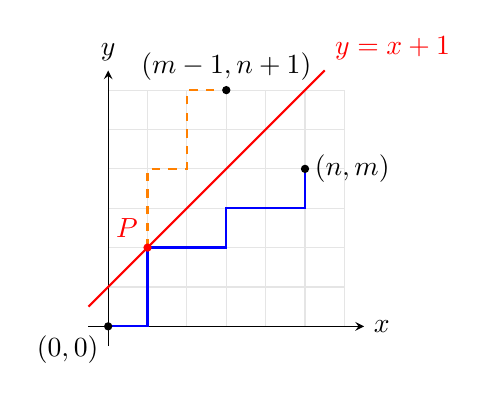
\begin{tikzpicture}[scale=0.5, >=stealth]
                % 绘制网格
                \draw[gray!20, thin] (0,0) grid (6,6);
                
                % 绘制坐标轴
                \draw[->] (-0.5,0) -- (6.5,0) node[right] {$x$};
                \draw[->] (0,-0.5) -- (0,6.5) node[above] {$y$};
                
                % 绘制限制线 y = x + 1
                \draw[red, thick] (-0.5,0.5) -- (5.5,6.5) node[above right] {$y=x+1$};
                
                % 定义关键点 (n=5, m=4) -> 反射点 (3, 6)
                \coordinate (A) at (0,0);
                \coordinate (B) at (5,4);
                \coordinate (Bprime) at (3,6);
                \coordinate (P) at (1,2); % 首次碰触点
                
                % 绘制到 B 的原始不合法路径
                % A -> P (正常段)
                \draw[blue, thick] (0,0) -- (1,0) -- (1,1) -- (1,2);
                % P -> B (未反射段)
                \draw[blue, thick] (1,2) -- (2,2) -- (3,2) -- (3,3) -- (4,3) -- (5,3) -- (5,4);
                
                % 绘制 P -> B' 的反射路径
                \draw[dashed, orange, thick] (1,2) -- (1,3) -- (1,4) -- (2,4) -- (2,5) -- (2,6) -- (3,6);
                
                % 标注点
                \fill (A) circle (3pt) node[below left] {$(0,0)$};
                \fill (B) circle (3pt) node[right] {$(n,m)$};
                \fill (Bprime) circle (3pt) node[above] {$(m-1,n+1)$};
                \fill[red] (P) circle (3pt) node[above left] {$P$};
            \end{tikzpicture}
        \end{column}
    \end{columns}



\end{frame}
\begin{frame}{反射容斥：旋转 $45^\circ$}
    在顺时针旋转 $45^\circ$ 再关于 $x$ 轴镜像后的图上想象这个过程或许会更容易。此时，不合法的路径是不碰到直线 $y=-1$ 的路径。

    
    \begin{center}
    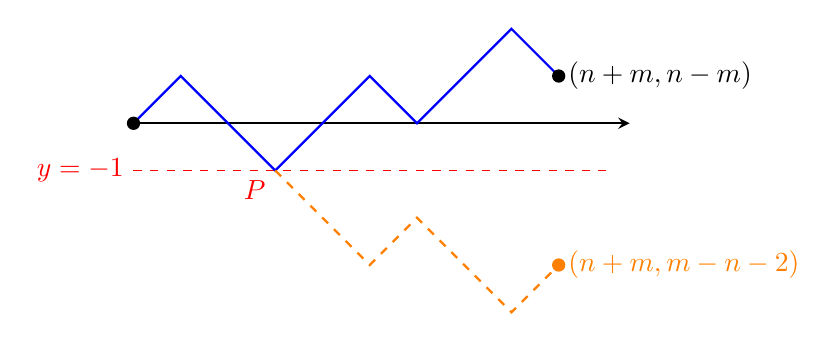
\begin{tikzpicture}[scale=0.6, >=stealth]
        % 绘制辅助水平线
        % \draw[gray!20, thin] (0,-2) grid (10,4);
        \draw[dashed, red] (0,-1) -- (10,-1);
        \draw[->, thick] (0,0) -- (10.5,0); % node[right] {$step$};
        
        % 路径节点定义 (n=5, m=5,  Catalan 情况)
        \draw[blue, thick] (0,0) -- (1,1) -- (3,-1) -- (5,1) -- (6,0) -- (8,2) -- (9,1);
        
        % 反射段 (从第一次碰到 h=1 的点 P(1,1) 开始)
        % 假设我们要反射 P 之后的所有步骤
        \draw[dashed, orange, thick] (3,-1) -- (5,-3) -- (6,-2) -- (8,-4) -- (9,-3);
        
        % 标注起点终点
        \fill (0,0) circle (4pt);
        \fill (9,1) circle (4pt) node[right] {$(n+m, n-m)$};
        \fill[orange] (9,-3) circle (4pt) node[right] {$(n+m, m-n-2)$};
        \node[red, left] at (0,-1) {$y=-1$};
        \node[red, anchor=north east] at (3,-1) {$P$};
    \end{tikzpicture}
    \end{center}

    另外，这个容斥也可以推广到不碰到两条线的情况。
\end{frame}

\begin{frame}{卡特兰数}
    在前面的问题中考虑 $n=m$ 的特殊情况，此时方案数是 
    $$
    C_n=\binom{2n}{n}-\binom{2n}{n-1}=\frac{1}{2n+1}\binom{2n+1}{n}.
    $$
    
    这个数列被称为\textbf{卡特兰数}（Catalan Number），它也在很多其他问题中自然地出现：

    \begin{itemize}
        \item 长为 $2n$ 的合法括号序列数量
        \item $n$ 个 $1$ 和 $n$ 个 $-1$ 组成的满足所有前缀和都非负的序列数量
        \item $n$ 个点的儿子有序的二叉树数量
        \item $n+1$ 个点的儿子有序的多叉树数量
        \item $n$ 个元素的出栈序数量
        \item $n+2$ 边形的三角剖分数量
    \end{itemize}
\end{frame}
\begin{frame}{括号序列}
    一个括号序列长什么样子？我们考虑所有最外层的括号，就得到 $\mathcal A=(\mathcal A)(\mathcal A)\cdots (\mathcal A)$。或者，我们可以把除了第一个括号以外的看成一体，就得到 $\mathcal A=\{\epsilon\}+(\mathcal A)\mathcal A$（$\epsilon$ 代表空序列）。把这两个构造翻译成递推式就得到
    $$
    C_n=\sum_{k\ge 0}\sum_{(i_1+1)+\cdots+(i_k+1)=n}C_{i_1}\cdots C_{i_k},\quad C_n=[n=0]+\sum_{i+1+j=n}C_{i}C_j.
    $$
    更好的做法是翻译成生成函数：
    $$
    C(x)=\frac{1}{1-xC(x)},\quad C(x)=1+xC(x)^2.
    $$

    也可以翻译成区间 dp，比如 [CSP-S 2021] 括号序列（不过这个题稍微复杂一点点）。
\end{frame}
\begin{frame}{括号序列与 $\pm 1$ 序列}
    我们把 $($ 看成 $+1$，$)$ 看成 $-1$，那么括号序列就一一对应由 $n$ 个 $+1$ 和 $n$ 个 $-1$ 组成的序列。这个转换是非常常用的。
    \begin{theorem}
        括号序列合法当且仅当对应的 $\pm 1$ 序列的任何前缀和都非负。
    \end{theorem}
    这样我们就建立了这两个组合类之间的双射。
\end{frame}
\begin{frame}{数列与格路径}
    另一方面，我们也经常把数列按照如下方式转化成格路径：从 $(0,0)$ 出发，逐个考虑 $i=1,\ldots,n$，遇到 $a_i$ 就走一步向量 $(1,a_i)$。例如，$+1,+1,-1,+1,-1,-1,+1,-1$ 对应下图所示的路径：
    \begin{columns}[T,onlytextwidth]
        \begin{column}{0.5\textwidth}
    \begin{center}
        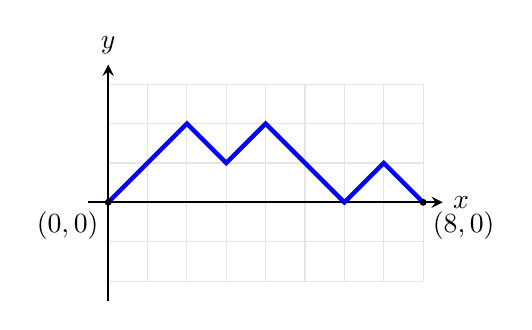
\begin{tikzpicture}[scale=0.5, >=stealth]
            % 1. 绘制背景网格 (使用浅灰色以免抢戏)
            \draw[gray!20, thin] (0,-2) grid (8,3);
        
            % 2. 绘制坐标轴
            \draw[->, thick] (-0.5,0) -- (8.5,0) node[right] {$x$};
            \draw[->, thick] (0,-2.5) -- (0,3.5) node[above] {$y$};
        
            % 3. 绘制路径 (示例序列: +1, +1, -1, +1, -1, -1, -1, +1)
            % 终点回到 (8,0)，中间有正有负
            \draw[blue, ultra thick] (0,0) 
                -- (1,1) 
                -- (2,2) 
                -- (3,1) 
                -- (4,2) 
                -- (5,1) 
                -- (6,0) 
                -- (7,1) 
                -- (8,0);
        
            % 4. 突出显示某一个步作为“向量”的示例
            % 选取第三步 (2,2) -> (3,1) 为例
            % \draw[->, red, thick] (2,2) -- (3,1); % node[midway, above right, scale=0.8] {$\vec{v}_3 = (1, a_3)$};
            % \draw[dashed, red!50] (2,2) -- (3,2) -- (3,1);
            % \node[red, scale=0.7] at (2.5, 2.2) {$1$};
            % \node[red, scale=0.7] at (3.3, 1.5) {$a_3$};
        
            % 5. 标注起点和终点
            \fill (0,0) circle (2.5pt) node[below left] {$(0,0)$};
            \fill (8,0) circle (2.5pt) node[below right] {$(8, 0)$};
        
            % 6. 在路径上方标注部分 a_i 符号（可选，增加直观度）
            % \node[blue, above left, scale=0.7] at (0.5, 0.5) {$a_1=+1$};
            % \node[blue, above left, scale=0.7] at (1.5, 1.5) {$a_2=+1$};
            % \node[blue, below right, scale=0.7] at (6.5, -0.5) {$a_7=-1$};
        \end{tikzpicture}
    \end{center}
    \end{column}
    \begin{column}{0.5\textwidth}
        \vspace{2em}
    记 $s_i$ 为数列的前缀和，则容易发现 $x=i$ 处的高度为 $s_i$。这也说明了图上两个点 $(i,s_i)$ 和 $(j,s_j)$ 之间的高度差对应数列的区间和 $s_j-s_i=\sum_{j<k\le i}a_k$。
    \end{column}
    \end{columns}

    所有前缀和都非负对应着不触碰 $y=-1$。这样，我们就建立起了 $\pm 1$ 序列与先前讨论的格路径之间的双射。
\end{frame}
\begin{frame}{组合直观}
    通过前面两个双射，我们证明了括号序列与 $\pm 1$ 序列的数量都是卡特兰数，所以先前对括号序列建立的递推式也就对应着卡特兰数的递推式。

    然而不同的组合结构带给人的直观感受是不同的！对于 $\pm 1$ 序列，我们几乎没有任何直观；对于括号序列，我们有序列分解的直观；对于格路径，我们有图像的直观。另外，前一页中的格路径似乎比之前旋转 $45^\circ$ 之前的格路径更加直观。
    
    事实上，我们也很容易对格路径建立先前对括号序列建立的递推：只需要考虑每一次触碰 $y=0$ 而分成的若干段即可。
\end{frame}
\begin{frame}{Raney 引理}
    我们还有另一个方法来得到卡特兰数的封闭形式，这需要 Raney 引理：

    \begin{lemma}[Raney 引理]
        对于一个和为 $1$ 的整数序列，其所有循环移位中恰好有一个满足：所有前缀和都是正的
    \end{lemma}
    它有一个（我们暂时用不到的）推广如下：
    \begin{lemma}[推广的 Raney 引理]
        对于一个和为 $\ell$ 且所有元素都 $\le 1$ 的整数序列，其所有循环移位中恰好有 $\ell$ 个满足：所有前缀和都是正的
    \end{lemma}
\end{frame}
\begin{frame}{证明}
    循环移位可以通过把序列复制一遍来处理。也就是说如果我们令 $a_{n+i}=a_i$，那么循环移位 $t$ 后得到的序列就是 $a[t+1,n+t]$。我们现在可以把复制一遍的序列画成格路径：
    \begin{center}
        \begin{tikzpicture}[scale=0.5, >=stealth]
            % 1. 绘制背景网格
            \draw[gray!20, thin] (0,-1) grid (14,3);
        
            % 2. 绘制坐标轴
            \draw[->, thick] (-0.5,0) -- (14.5,0) node[right] {$x$};
            \draw[->, thick] (0,-1.5) -- (0,3.5) node[above] {$y$};
        
            % 3. 绘制蓝色主路径并标记点
            % 使用 plot[mark=*] 可以一次性画出线和点，非常干净
            \draw[blue, thick, mark=*, mark size=1.5pt, mark options={fill=blue}] 
                plot coordinates {
                    (0,0) (1,2) (2,-1) (3,1) (4,0) (5,2) (6,2) (7,1) 
                    (8,3) (9,0) (10,2) (11,1) (12,3) (13,3) (14,2)
                };
    
            % 4. 在 x=7 处画虚线切分
            \draw[dashed, red, thick] (7,-1.5) -- (7,3.5) node[above] {$x=n$};

            \draw[red,thick] (2,-1) node[below] {\tiny 唯一可行起点};
    
            % 5. 标注关键坐标
            % \node[below left] at (0,0) {\tiny $(0,0)$};
            % \node[below right, red] at (7,1) {\tiny $(n, S_n)$};
            % \node[above right] at (14,2) {\tiny $(2n, 2S_n)$};
    
        \end{tikzpicture}
    \end{center}
    现在， $[i+1,n+i]$ 这一段区间对应的格路径相当于以 $(i,s_i)$ 为起点、以 $(n+i,s_{n+i})$ 为终点的格路径，而所有前缀和均为正相当于过程中高度始终高于起点。那么显然有且仅有以那个最小的 $s_i$（相等的话认为 $i$ 大的小）为起点才能做到这一点。
\end{frame}
\begin{frame}{$\pm 1$ 序列：再探}
    我们需求的是所有前缀和非负，而 Raney 引理中是所有前缀和 $>0$。我们可以通过在序列开头加一个 $1$ 来处理这个问题。也就是说我们考虑双射：$n$ 个 $+1$ 和 $n$ 个 $-1$ 组成的所有前缀和非负的序列 $\leftrightarrow$ 由 $n+1$ 个 $+1$ 和 $n$ 个 $-1$ 组成的所有前缀和 $>0$ 的序列。

    对于新的问题，Raney 引理告诉我们可以将所有可能的 $\binom{2n+1}{n}$ 个序列按照循环移位划分等价类，而每个等价类恰好贡献一种合法方案。由于 $\gcd(n+1,n)=1$，每个等价类的大小都是 $2n+1$（也就是说一个序列的所有循环移位都是不同的），除法原理就告诉我们合法方案数为
    $$
    \frac{1}{2n+1}\binom{2n+1}{n}.
    $$
\end{frame}
\begin{frame}{二叉树}
    二叉树具有自然的左子树-根-右子树结构，也就是 $
\mathcal A=\{\epsilon\}+\begin{array}{c}
\bullet \\
/ \quad \backslash \\
\mathcal A \quad \mathcal A
\end{array}
$，所以二叉树和合法括号序列有相同的递推式。又因为初值也相同，所以二叉树的数量也是卡特兰数。

我们也可以把这个结构与括号序列的结构进行对应，据此得到一个双射：记 $S[T]$ 为树 $T$ 映射到的括号序列，则

$$
S\left[\begin{array}{c}
    \bullet \\
    / \quad \backslash \\
    L \quad R
    \end{array}\right]=(S[L])S[R],\quad S[\epsilon]=\epsilon.
$$

另外，我们还需要注意 $n$ 个点的二叉树与有 $n$ 个\textbf{内点}的满二叉树\footnote{这里满二叉树指所有非叶结点都有两个儿子的二叉树}的一一对应（内点即左右子树都非空的节点）：想象在每个非内点下面长叶子来变成内点

\end{frame}
\begin{frame}{多叉树}
    通过枚举儿子数量，我们得到
    $$
    \mathcal A=\begin{array}{c}\bullet\end{array}+\begin{array}{c}
        \bullet \\
        |  \\
        \mathcal A
        \end{array}
        +\begin{array}{c}
        \bullet \\
        / \quad \backslash \\
        \mathcal A \quad \mathcal A
        \end{array}
        +\begin{array}{c}
            \bullet \\
            / \  |\  \backslash \\
            \mathcal A \  \mathcal A \ \mathcal A
            \end{array}
        +\cdots
    $$
    那么具有 $n+1$ 个点的多叉树和长为 $2n$ 的括号序列有相同的递推式。我们同样可以据此得到一个双射：
    $$
    S\left[\begin{array}{c}
        \mathbf{\bullet} \\
        / \ \cdots\  \backslash \\
        T_1\ \ \cdots \ \  T_k
        \end{array}\right]=(S[T_1])\cdots(S[T_k])
    $$
\end{frame}
\begin{frame}{出栈序}
    维护一个栈 $S$ 和一个整数 $i=1$，在任意时刻可以 (i) 如果 $i\le n$，则将 $i$ 入栈，并令 $i\gets i+1$ 或者 (ii) 如果栈非空，则弹出当前栈顶。等到无法继续操作时，按照出栈的顺序可以得到一个排列。这就是 $1,\ldots,n$ 的出栈序。这是一个不太常用的模型，因为它不够直观而且分析比较复杂。
    
    考虑最后一次操作，这一定是一个出栈。假设这次出栈的元素是 $x$，那么考虑 $x$ 的入栈时刻 $t$，则在 $t$ 时刻结束后栈中一定只有 $x$ 自己（否则 $x$ 无法最后出栈）。因此，出栈序可以按顺序划分成三部分：$[1,x)$ 的出栈序、$(x,n]$ 的出栈序、$x$。这又是一个卡特兰数类型的递归。

    另一方面，我们可以注意到操作序列与出栈顺序的联系。由于每个元素出入栈各一次，序列的长度必然是 $2n$。因此，上面的分析也给出了操作序列的划分，于是出栈序与操作序列一一对应。而操作序列天然对应一个括号序列（入栈/出栈分别对应左/右括号）。
\end{frame}
\begin{frame}
    按照前面的分析，我们还可以给出和二叉树的一个双射：我们给二叉树按照中序遍历编号，则出栈序对应一个后序遍历。我们知道中序遍历+先/后序遍历可以唯一确定一棵二叉树。

    最后，出栈序等价于 312 禁子排列，即不存在 $i<j<k$ 但是 $\pi_j<\pi_k<\pi_i$ 这种模式的排列。因为如果我们考虑 $\pi_n$，则 $k=n$ 的限制的影响是 $(\pi_n,n]$ 必须出现在 $[1,\pi_n)$ 右边，然后剩下的限制只有这两块内部的限制。
\end{frame}
\begin{frame}{多边形三角剖分}
    顺时针给所有顶点编号。考虑最终剖分中 $1-n$ 这条边在其所在的三角形中的对点 $i$，则此三角形划分出了两个子结构，规模分别为 $i$ 和 $n-i+1$。这是 $C_{n+2}$ 满足的递归。

    可以据此设计到二叉树的双射：每个三角形视为一个点，与相邻的三角形连边。事实上，这就是平面图转对偶图。
\end{frame}
\begin{frame}{根据组合结构 dp}
    组合结构往往具有自然的子结构。最常见的包括：

    \begin{itemize}
        \item 序列：前缀/区间
        \item 树：子树/链
        \item 集合：子集
        \item 网格：1/2-side 子矩形；轮廓线
        \item DAG：子 DAG（拓扑序）
    \end{itemize}
\end{frame}
\begin{frame}{[CSP-S 2021] 括号序列}
\end{frame}
\begin{frame}{利用乘法原理 dp}
    合适地刻画子问题，使得每种子问题对后续状态的转移系数都相同。

    例：[CSP-S 2025] 员工招聘
\end{frame}

\begin{frame}
    做法零：将 (前 $i$ 个人，要求形成的部分排列为 $P$，的部分排列数量) 作为子问题。$\tilde O(n!)$

    做法一：将 (前 $i$ 个人，要求构成的集合为 $S$、目前未录用的人数为 $j$，的部分排列数) 作为子问题。$\tilde O(2^n)$。这个刻画对大部分排列类计数都适用。

    做法二（伪）：将 (前 $i$ 个人，要求目前未录用的人数为 $j$、$c>j$ 的人中还没放的人数为 $k$，的部分排列数) 作为子问题。然而，这样不能转移，因为无法知道下一个位置不录用时再下一个位置的候选人数会如何变化。

    做法二（真）：上一个做法中，“无法知道下一个位置不录用时再下一个位置的候选人数会如何变化”的原因如下：假设目前不录用人数是 $j$，而之前可能已经录用了一些 $c=j+1$ 的人，但这个人数没有在状态中记录。所以我们可以考虑把 $c=j+1$ 的人等到最后再一起放了。也就是将 (前 $i$ 个人，要求目前未录用的人数为 $j$、$c>j$ 的人中还没放的人数为 $k$、只确定了 $c\le j$ 的人的位置，形成的部分排列数) 作为子问题。这个技巧也称为“贡献延后计算”。
\end{frame}
\begin{frame}{另一个视角}
    假设我们先钦定了所有位置的录取情况，那么如何计算方案数？对于一个录取的位置，必须有 $s_i=1$ 且 $c_{\pi_i}>f_i$，其中 $f_i$ 为 $i$ 前面的未录取人数；对于一个未录取的位置，需要 $s_i=0$ 或者 $c_{\pi_i}\le f_i$。那么相当于每个位置有限制 $c_{\pi_i}>f_i$ 或者 $c_{\pi_i}\le f_i$ 或者无限制。

    现在来考虑子问题：(i) 如果只有某一种限制怎么做？(ii) 如果只有某两种限制怎么做？(iii) 怎么把某一种限制用另外两种限制表示？

    如果把无限制表示成 $[c_{\pi_i}>f_i]+[c_{\pi_i}\le f_i]$，那就能得到上一页中的做法。如果把 $[c_{\pi_i}>f_i]$ 表示成 $1-[c_{\pi_i}\le f_i]$，那么就得到另一种做法，也就是容斥。

    最后，可以在 dp 中枚举所有位置的录取情况。    
\end{frame}

\begin{frame}{生成函数初步}
    这里主要介绍怎么用生成函数（Generating Function, GF）处理序列（假设已经得到序列的某些性质，如递推关系等）。事实上更多情况下可以直接对着问题的结构写出生成函数，而无需额外经过一步 dp 转化。绝大多数的推式子问题都有办法用生成函数处理。但需要强调的是生成函数\textbf{并非万能}，不应忽视其他的技巧和组合意义。在使用生成函数之前先做一些基本的处理往往能简化推导。

    最基本和主要的手段就是把需要处理的序列 $(f_i)$ 挂到幂级数 $\sum_{i\ge 0}f_i a_i x^i$ 上去，其中 $a_i$ 是自己选定的另一组系数，通常是 $1$（普通生成函数，\textbf{O}rdinary GF）或 $1/i!$（指数生成函数，\textbf{E}xponential GF）。这样导出的幂级数几乎总是比序列容易处理的。注意在实践中一般需要假设 $x\approx 0$ 是一个小量。我们后面说的“幂级数”和“生成函数”都是指的同一个东西。

    记 $[x^n]F(x)$ 为幂级数 $F(x)$ 的第 $n$ 次项系数。在上下文清楚时，有时我们也用 $f_n$ 代表这个事情。（注意：如果上面挂到幂级数上时使用了非 $1$ 的 $a_i$，那么这里的 $f_n$ 代表上面 $\sum_{n\ge 0}f_na_nx^n$ 中的 $f_na_n$ 而不是 $f_n$ 本身，后同）
\end{frame}
\begin{frame}{运算法则 I}
    可以对幂级数与它的封闭形式做同样的运算来得到以下的对应关系：

    线性运算 $H(x)=aF(x)+bG(x)$ 对应 $h_n=af_n+bg_n$

    卷积 $H(x)=F(x)G(x)$ 对应 $h_n=\sum_{i=0}^n f_ig_{n-i}$。更一般地，
    $$
    [x^n]F_1(x)F_2(x)\cdots F_m(x)=\sum_{i_1+i_2+\cdots+i_m=n}([x^{i_1}]F_1(x))([x^{i_2}]F_2(x))\cdots ([x^{i_m}]F_m(x)).
    $$

    求导 $H(x)=F'(x)$ 对应 $h_n=(n+1)f_{n+1}$。
\end{frame}
\begin{frame}{求导}
    导数有几个不同的记号，$f'(x)$、$\frac{\mathrm{d}}{\mathrm{d}x} f(x)$、$\mathbf D f(x)$ 都可以用来代表求导。如果需要反复求导（高阶导数），那么可以用 $f'''(x)$、$f^{(k)}(x)$、$\frac{\mathrm{d^k}}{\mathrm{d}x^k} f(x)$、$\mathbf D^k f(x)$ 这些记号。

    我们做的所有操作都是\textbf{形式上的}。你只需要（熟练）记住以下这些事实：
    \begin{itemize}
        \item 运算性质 $(af(x)+bg(x))'=af'(x)+bg'(x)$，$(f(x)g(x))'=f'(x)g(x)+f(x)g'(x)$，$(f(g(x)))'=f'(g(x))g'(x)$
        \item 初等函数的导数 $(x^{\alpha})'=\alpha x^{\alpha-1},\ (\ln x)'=x^{-1},\ (e^x)'=e^x$
    \end{itemize}
    下面是几个练习。这些结果也是有价值且值得记住的：
    \begin{itemize}
        \item 常数的导数是 $0$
        \item $(f(x)/g(x))'=\frac{f'(x)g(x)-f(x)g'(x)}{g(x)^2}$
        \item $(\log f(x))'=\frac{f'(x)}{f(x)}$
        % \footnotetext{这里 $\log$ 和 $\ln$ 指的是一个东西，这是常见的做法。在计算机科学中的另一个常见做法是默认 $\log=\log_2$。}
        \item $(e^{f(x)})'=f'(x)e^{f(x)}$
        \item $(fg)^{(k)}=\sum_i \binom{k}{i}f^{(i)}g^{(k-i)}$
    \end{itemize}
\end{frame}
\begin{frame}{运算法则 II}
    $H(x)=x^mF(x)$ 对应移位 $h_n=f_{n-m}$。注意：尽量不要让你的式子中出现\textbf{负下标项}，所以在 $m$ 为负时要小心。。

    $H(x)=\frac{1}{1-x}F(x)$ 对应前缀和 $h_n=\sum_{i\le n}f_i$

    $H(x)=(1-x)F(x)$ 对应差分 $h_n=f_n-f_{n-1}$

    $H(x)=\vartheta F(x)\overset{\mathrm{def}}{=}xF'(x)$ 对应原地的求导 $h_n=nf_n$

    $H(x)=F(x)\bmod (x^k-1)$ 对应 $h_r=\sum_n f_{kn+r}$。（事实上模一般的 $Q(x)$ 相当于按一个线性递推累加系数）

    $H(x)=x^kF^{(k)}(x)$ 对应 $h_n=n^{\underline{k}}f_n$

    $H(x)=(x\mathbf D)^kF(x)$ 对应 $h_n=n^k f_n$。然而，$(x\mathbf D x)^k$ 一般没有好的封闭形式（虽然 $(x\mathbf D)^k=\sum_i {k\brace i}x^i\mathbf D^i$）
\end{frame}
\begin{frame}{最重要的一些生成函数}
    下面几个恒等式是应该（双向）记住的，因为它们实在是太常见了。
    $$
    \begin{aligned}
    &(1+x)^{\alpha}=\sum_{n\ge 0}\binom{\alpha}{n}x^n,\quad \ln\left(\frac{1}{1-x}\right)=\sum_{n\ge 1}\frac{x^n}{n}\quad e^x=\sum_{n\ge 0}\frac{x^n}{n!}\\
    \end{aligned}
    $$
    第一个恒等式——也就是二项式定理——的一些特殊情况也是值得记忆的（证明它们！）：
    $$
    \begin{aligned}
    \frac{1}{(1-x)^k}=\sum_{n\ge 0}\binom{n+k-1}{n}x^n,\quad\frac{x^k}{(1-x)^{k+1}}=\sum_{n\ge 0}\binom{n}{k}x^n,\quad \frac{1}{\sqrt{1-4x}}=\sum_{n\ge 0}\binom{2n}{n}x^n
    \end{aligned}
    $$
\end{frame}
\begin{frame}{代入}
    $x$ 可以代入为任何 $\approx 0$ 的东西（有些时候还可以代入别的东西\footnote{在 OI 里，你基本可以认为是\textit{任何东西}}，取决于\textbf{收敛半径}）。在生成函数的语境下，$\approx 0$ 的东西指的就是任何\textbf{常数项为} $\mathbf 0$ 的幂级数。

    直接的例子：
    $$
    F(x^k)=\sum_{n\ge 0}f_nx^{nk},\quad F(rx)=\sum_{n\ge 0}f_nr^nx^n.
    $$
    复杂一点的例子：
    $$
    \sum_{n\ge 0}\left(\frac{x}{1-x}\right)^n=\frac{1}{1-\frac{x}{1-x}}=\frac{1-2x}{1-x}
    $$
    代值的例子：把 $x=1$ 和 $x=-1$ 分别代入 $(1+x)^n$。把 $|r|<1$ 的 $r$ 代入 $1/(1-x)^k$。 
\end{frame}
\begin{frame}{使用例}
    化简范德蒙德卷积 $\sum_i\binom{r}{i}\binom{s}{n-i}$。我们只需要乘上 $x^n$ 然后对 $n$ 求和，化简得到的生成函数，最后再提取 $[x^n]$。也就是
    $$
    [x^n]\sum_n x^n\binom{r}{i}\binom{s}{n-i}.
    $$
    用这个方法化简（注意：你需要决定对哪个变量做我们前面说的事情）
    $$
    \sum_{k}\binom{l}{m+k}\binom{s+k}{n}(-1)^k,\quad \sum_{-q\le k\le l}\binom{l-k}{m}\binom{q+k}{n},\quad     \sum_{k\ge 0}\binom{n+k}{m+2k}\binom{2k}{k}\frac{(-1)^k}{k+1}.
    $$
    （然而问题 8 没有办法直接这样做...但是有另外的技巧可以做...）
    
    试着对下面的式子做同样的事情（我们一会再来教大家怎么提取这种系数）
    $$
    \sum_{k\le n}\binom{n-k}{k}(-1)^k
    $$
\end{frame}
\begin{frame}{方程}
    对斐波那契数列的递推公式 $f_n=f_{n-1}+f_{n-2}$ 使用前面的方法。根据得到的方程解出生成函数。通过对生成函数求导，导出一个 $\sum_{i=0}^nf_if_{n-i}$ 的简化形式。
    
    对卡特兰数的递推公式 $C_n=\sum_{i=0}^{n-1}C_iC_{n-i-1}$ 使用前面的方法。据此导出卡特兰数的封闭形式。

    对错排的递推公式 $d_n=(n-1)(d_{n-1}+d_{n-2})$、$d_n=nd_{n-1}+(-1)^n$ 使用前面的方法（试试 OGF 和 EGF，也就是分别乘 $x^n$ 和 $x^n/n!$）。
\end{frame}

\begin{frame}{回顾}
    我们看看如何用生成函数处理以前的一些问题。这里，我们可以先只关心生成函数的封闭形式，等会再考虑如何计算。
    $$
    \sum_{0\le i\le n}\mathrm{Fib}_i,\quad \sum_{1\le i_1\le i_2\le\cdots\le i_m\le n} 1,\quad     \sum_{i=0}^n r^ii^k,\quad \sum_i\binom{n}{i}r^ia_{i\bmod k}.
    $$
\end{frame}
\begin{frame}{趣味问题}
    $$
    \sum_i\binom{n}{i}r^{\lfloor i/k\rfloor}
    $$

    （假设 $r^{1/k}$ 和 $\omega_k$ 都不存在）。感觉是不太广为人知的东西。

    可以使用一些深刻的背景知识将其扩展到 $\langle H(x),F(x)\rangle$，其中 $H$ 是某个稀疏多项式，$F(x)$ 是任意线性递推，$\langle \cdot,\cdot\rangle$ 表示系数点积。
\end{frame}
\begin{frame}{计算}
    得到一个生成函数的封闭形式后，如何用于计算第 $n$ 项或者前 $n$ 项？下面是几种常见的方法：
    \begin{itemize}
        \item 对于比较简单的情况，可以直接使用前面的常见级数展开来得到系数。
            \begin{itemize}
                \item 这里可能能直接得到封闭形式，也可能得到一个卷积求和
            \end{itemize}
        \item 对于有理分式，可以分式分解，或者使用线性递推
        \item 使用 FFT 来进行各种多项式运算
        \item 使用暴力来进行各种多项式运算
        \item 通过求导等手段得到递推式
        \item 拉格朗日反演
    \end{itemize}
\end{frame}
\begin{frame}{分式分解}
    对于 $P(x)/Q(x)$（$P,Q$ 都是多项式）的形式，可以先将其变成 $P(x)\ \mathrm{div}\ Q(x)+\frac{P(x)\bmod Q(x)}{Q(x)}$。然后可以假设 $\deg P<\deg Q$。（有人不会多项式除法吗？）

    真分式总是有如下的分解：
    $$
    \frac{P(x)}{\prod{(a_ix+b_i)^{k_i}}}=\sum_i\sum_{j=1}^{k_i}\frac{c_{ij}}{(a_ix+b_i)^{j}}.
    $$

    可以待定系数计算 $c_{ij}$。当 $k_i=1$ 时，有更方便的算法。两侧同乘 $a_ix+b_i$，然后代入 $x_i=-b_i/a_i$ 就得到
    $$
    \frac{P(x_i)}{\prod_{j\ne i}(a_jx_i+b_j)^{k_j}}=c_{i1}
    $$
\end{frame}
\begin{frame}{线性递推}
    对于有理真分式 $F(x)=P(x)/Q(x)$，两侧乘 $Q(x)$ 得到 $F(x)Q(x)=P(x)$。展开卷积就得到线性递推。

    使用分式分解即可得到所有线性递推的相关结论。例如，你现在应该能够自行推出
    $$
    f_n=\sum_{i=1}^k a_if_{n-i}+r^n(\sum_{i=0}^m b_in^{\underline{i}})
    $$
    的生成函数的封闭形式。

    我们现在有非常简单的 $O(\mathbf{M}(m)\log n)$ 算法来得到一个有理分式的第 $n$ 次项系数：注意到 $Q(x)Q(-x)$ 只有偶数项有值，考虑 $[x^n]\frac{P(x)}{Q(x)}=[x^n]\frac{P(x)Q(-x)}{Q(x)Q(-x)}$，后者只与分子的奇数/偶数次项有关（取决于 $n\bmod 2$），据此我们可以将 $n$ 减半，而分式的规模保持不变。
\end{frame}
\begin{frame}{$O(n^2)$ 多项式运算 I}
    下面的 $n,m$ 都指多项式的\textbf{项数}而不是次数。对 $F(x)$ 用 $n$，对 $G(x)$ 用 $m$。 
    \begin{itemize}
        \item  可以在线性时间内计算 $aF(x)+bG(x)$、$x^mF(x)$、$F'(x)$、$\int_0^x F(t)\mathrm{d}t$。
        \item 可以在 $O(nm)$ 时间内计算 $F(x)G(x)$。所以当 $\min(n,m)$ 非常小时复杂度优秀
        \item 可以在 $O(m(\deg F-\deg G))$ 时间内计算 $F(x)\ \mathrm{div}\  G(x)$ 和 $F(x)\bmod G(x)$
        \item 后两者可以用 FFT 做到 $O(N\log N)$，其中 $N=\max(\deg F,\deg G)$
    \end{itemize}
\end{frame}
\begin{frame}{$O(n^2)$ 多项式运算 II}
    假设 $F$ 的\textbf{项数} $<m$，那么可以在 $O(nm)$ 时间内计算下列级数的前 $n$ 项（可以假设 $m\le n$，为什么？）。实践中 $m$ 经常很小，此时这种暴力的复杂度非常优秀。
    \begin{itemize}
        \item $G=F^{-1}H$（需求 $f_0\ne 0$）：也就是 $G\cdot F=H$，直接展开卷积就得到一个递推式
        \item $G=\ln F$（需要 $f_0=1$）：两侧求导得到 $G'=F'/F$，也就是 $FG'=F'$，展开卷积就得到一个递推式。初值 $g_0=0$。
        \item $G=e^F$（需要 $f_0=0$）：两侧求导得到 $G'=F'G$，展开卷积得到递推式。初值 $g_0=1$。
        \item $G=F^k$：两侧求导得到 $G'=kF'G/F$，也就是 $FG'=kF'G$，展开卷积得到递推式。初值 $g_0=f_0^k$。
        \item 练习：假设 $F$ 是分子分母项数都不超过 $m$ 的有理分式，在 $O(nm)$ 时间内求出 $F$ 的前 $n$ 项。
    \end{itemize}

    以上都可以用 FFT 做到 $O(n\log n)$。注意到在 $m$ 为常数时，这还不如上面的做法。
\end{frame}
\begin{frame}{更多技巧}
    还有值得再讲一个专题的例子和技巧，然而这里时间不够。
\end{frame}
